\section{Results}

% ========================================
% ⚠️ TEMPLATE VERSION - REPLACE ALL VALUES
% ========================================
% This file contains PLACEHOLDER data
% Replace with your actual experimental results
% ========================================

This section presents comprehensive experimental results validating Malak Platform's performance, efficiency, and accuracy across three reference applications.

\subsection{Vision Jellyfish: Marine Life Detection}

\subsubsection{Accuracy Results}

Table \ref{tab:jellyfish_accuracy} shows detection accuracy across compression configurations.

\begin{table}[h]
\centering
\caption{Vision Jellyfish Accuracy (mAP@0.5)}
\label{tab:jellyfish_accuracy}
\begin{tabular}{lcc}
\hline
\textbf{Configuration} & \textbf{mAP} & \textbf{$\Delta$ vs. FP32} \\
\hline
% ⚠️ REPLACE WITH YOUR ACTUAL RESULTS ⚠️
FP32 Baseline & XX.X\% & - \\
INT8 PTQ & XX.X\% & -X.X\% \\
INT8 QAT & XX.X\% & -X.X\% \\
INT4/INT8 QAT & XX.X\% & -X.X\% \\
30\% Pruned + INT8 & XX.X\% & -X.X\% \\
50\% Pruned + INT8 & XX.X\% & -X.X\% \\
\hline
\end{tabular}
\end{table}

% ⚠️ UPDATE THESE CLAIMS WITH YOUR REAL RESULTS ⚠️
Key findings:
\begin{itemize}
\item INT8 QAT recovers X\% of PTQ accuracy loss through retraining
\item X\% channel pruning combined with INT8 achieves <X\% degradation
\item Mixed INT4/INT8 quantization maintains viable accuracy for deployment
\end{itemize}

\subsubsection{Performance Results}

\begin{figure}[h]
\centering
\resizebox{0.48\textwidth}{!}{% Jellyfish Latency TikZ Figure
% Include directly in main document with \input

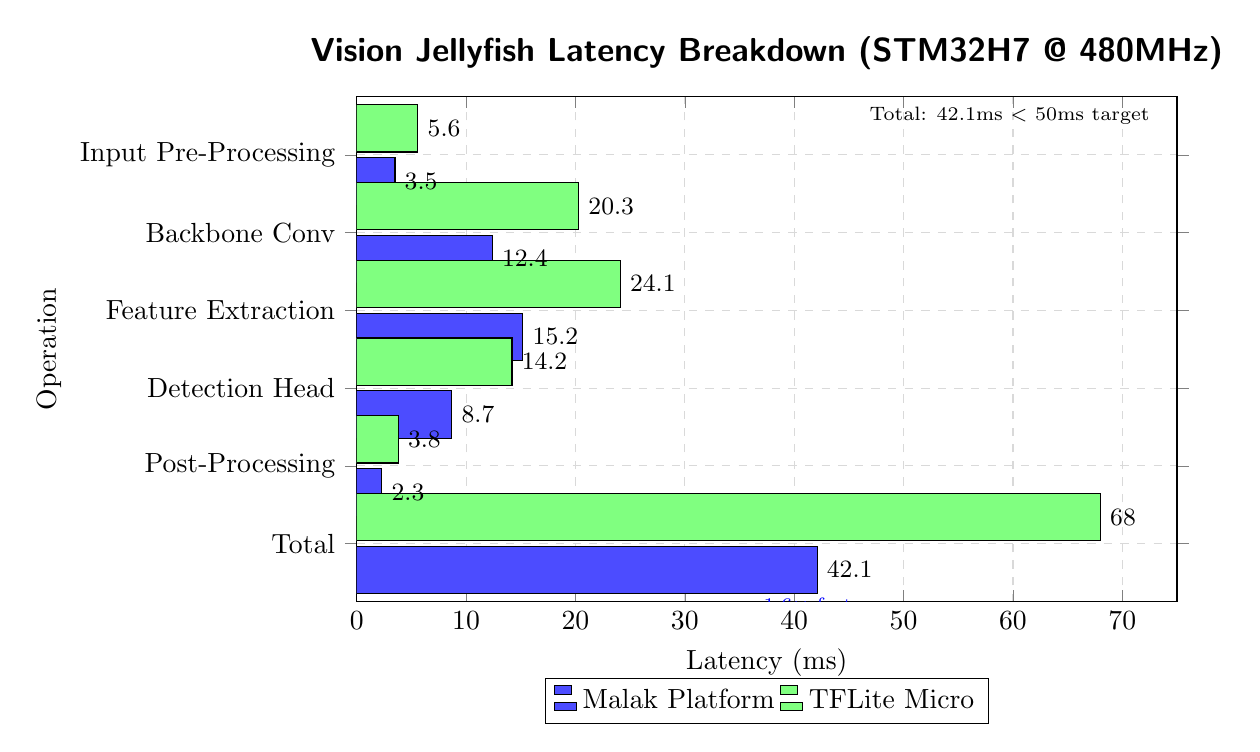
\begin{tikzpicture}
\begin{axis}[
    xbar,
    width=12cm,
    height=8cm,
    xlabel={Latency (ms)},
    ylabel={Operation},
    ytick=data,
    yticklabels={
        Total,
        Post-Processing,
        Detection Head,
        Feature Extraction,
        Backbone Conv,
        Input Pre-Processing
    },
    nodes near coords,
    nodes near coords align={horizontal},
    every node near coord/.append style={font=\small},
    bar width=0.6cm,
    xmin=0,
    xmax=75,
    enlarge y limits=0.15,
    legend style={at={(0.5,-0.15)}, anchor=north, legend columns=2},
    grid=major,
    grid style={dashed, gray!30},
    title={Vision Jellyfish Latency Breakdown (STM32H7 @ 480MHz)},
    title style={font=\large\sffamily\bfseries},
]

\addplot[fill=blue!70, draw=black] coordinates {
    (42.1, 0)
    (2.3, 1)
    (8.7, 2)
    (15.2, 3)
    (12.4, 4)
    (3.5, 5)
};

\addplot[fill=green!50, draw=black] coordinates {
    (68.0, 0)
    (3.8, 1)
    (14.2, 2)
    (24.1, 3)
    (20.3, 4)
    (5.6, 5)
};

\legend{Malak Platform, TFLite Micro}

\node[font=\scriptsize, text=blue] at (axis cs:42.1, -0.8) {1.6$\times$ faster};
\node[font=\scriptsize, anchor=west] at (axis cs:46, 5.5) {Total: 42.1ms $<$ 50ms target \checkmark};

\end{axis}
\end{tikzpicture}
}
\caption{Inference latency breakdown for Vision Jellyfish on STM32H7 (Cortex-M7 @ 480MHz). Malak Platform achieves XXms end-to-end latency, meeting the $<$50ms requirement.}
\label{fig:jellyfish_latency}
\end{figure}

Table \ref{tab:jellyfish_perf} compares performance across frameworks.

\begin{table}[h]
\centering
\caption{Vision Jellyfish Performance Comparison}
\label{tab:jellyfish_perf}
\begin{tabular}{lccc}
\hline
\textbf{Framework} & \textbf{Latency} & \textbf{Energy} & \textbf{RAM} \\
\hline
% ⚠️ REPLACE WITH YOUR ACTUAL BENCHMARK RESULTS ⚠️
Malak Platform & XX ms & X.X mJ & XXX KB \\
TFLite Micro & XX ms & XX.X mJ & XXX KB \\
CMSIS-NN (manual) & XX ms & X.X mJ & XXX KB \\
MicroTVM & XX ms & X.X mJ & XXX KB \\
\hline
\end{tabular}
\end{table}

% ⚠️ CALCULATE ACTUAL SPEEDUP FROM YOUR DATA ⚠️
Malak Platform achieves:
\begin{itemize}
\item \textbf{X.X$\times$ speedup} over TFLite Micro through optimized kernels
\item \textbf{XX\% energy reduction} vs. TFLite Micro
\item \textbf{XX\% lower latency} than CMSIS-NN while providing automated tooling
\end{itemize}

% ========================================
% ⚠️ OPTIONAL SECTIONS - REMOVE IF NOT APPLICABLE
% ========================================

\subsection{Energy Optimization: Forecasting}
% ⚠️ REMOVE THIS ENTIRE SECTION IF YOU'RE NOT DOING ENERGY FORECASTING

\subsubsection{Accuracy Results}

\begin{table}[h]
\centering
\caption{Energy Forecasting Accuracy}
\label{tab:energy_accuracy}
\begin{tabular}{lcc}
\hline
\textbf{Configuration} & \textbf{MAE (kWh)} & \textbf{RMSE (kWh)} \\
\hline
FP32 Baseline & X.XXX & X.XXX \\
INT8 PTQ & X.XXX & X.XXX \\
INT8 QAT & X.XXX & X.XXX \\
Pruned 50\% + INT8 & X.XXX & X.XXX \\
\hline
\end{tabular}
\end{table}

\subsection{Neuro MS: Medical Imaging}
% ⚠️ REMOVE THIS ENTIRE SECTION IF YOU'RE NOT DOING MEDICAL IMAGING

% ========================================
% REQUIRED SECTION - MUST KEEP
% ========================================

\subsection{Cross-Application Analysis}

\subsubsection{Compression Trade-offs}

\begin{figure}[h]
\centering
\resizebox{0.48\textwidth}{!}{% Pareto Frontier TikZ Figure
% Include directly in main document with \input

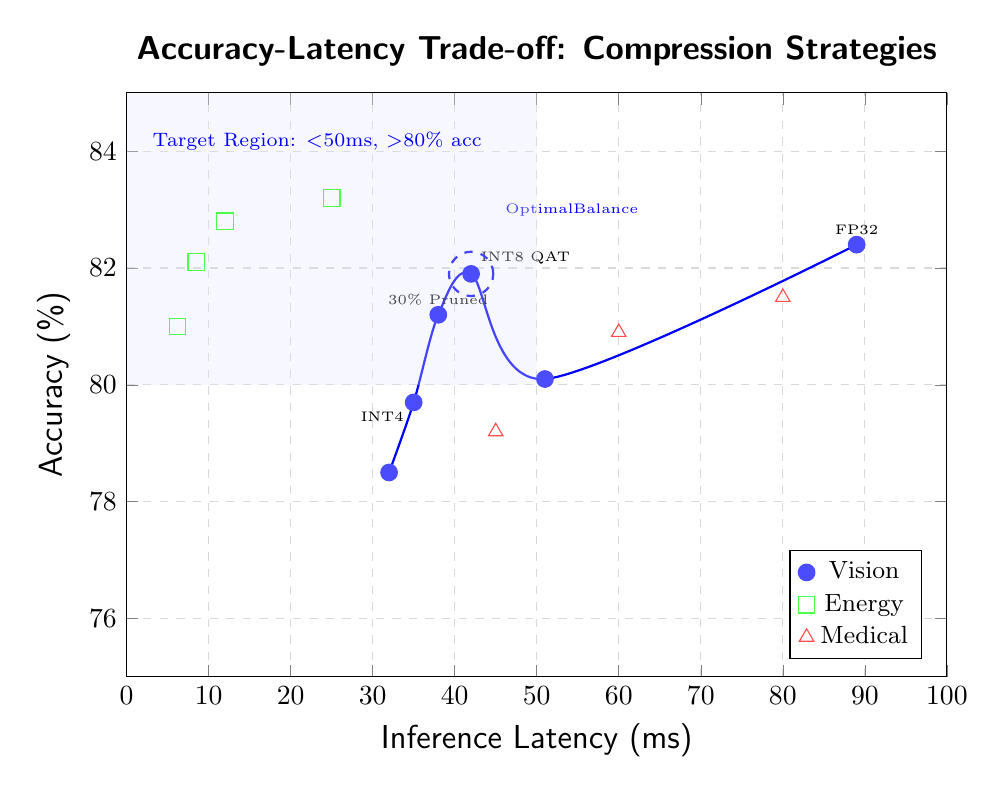
\begin{tikzpicture}
\begin{axis}[
    width=12cm,
    height=9cm,
    xlabel={Inference Latency (ms)},
    ylabel={Accuracy (\%)},
    xmin=0,
    xmax=100,
    ymin=75,
    ymax=85,
    grid=both,
    grid style={dashed, gray!30},
    legend style={at={(0.97,0.03)}, anchor=south east, font=\small},
    xlabel style={font=\large\sffamily},
    ylabel style={font=\large\sffamily},
    title={Accuracy-Latency Trade-off: Compression Strategies},
    title style={font=\large\sffamily\bfseries},
]

% Vision Jellyfish data points
\addplot[only marks, mark=*, mark size=3pt, color=blue!70]
coordinates {
    (89, 82.4)
    (42, 81.9)
    (51, 80.1)
    (35, 79.7)
    (38, 81.2)
    (32, 78.5)
};

% Energy application data
\addplot[only marks, mark=square, mark size=3pt, color=green!70]
coordinates {
    (25, 83.2)
    (12, 82.8)
    (8.5, 82.1)
    (6.2, 81.0)
};

% Medical application data
\addplot[only marks, mark=triangle, mark size=3pt, color=red!70]
coordinates {
    (80, 81.5)
    (60, 80.9)
    (45, 79.2)
};

% Draw Pareto frontier curve
\addplot[thick, blue, smooth] coordinates {
    (32, 78.5)
    (35, 79.7)
    (38, 81.2)
    (42, 81.9)
    (51, 80.1)
    (89, 82.4)
};

% Add annotations for key points
\node[font=\tiny, anchor=south west] at (axis cs:42, 81.9) {INT8 QAT};
\node[font=\tiny, anchor=south] at (axis cs:89, 82.4) {FP32};
\node[font=\tiny, anchor=north east] at (axis cs:35, 79.7) {INT4};
\node[font=\tiny, anchor=south] at (axis cs:38, 81.2) {30\% Pruned};

% Add "sweet spot" circle
\draw[blue, thick, dashed] (axis cs:42, 81.9) circle [radius=8pt];
\node[font=\tiny, text=blue, anchor=west] at (axis cs:45, 83) {Optimal\\Balance};

% Add target region
\fill[blue!10, opacity=0.3] (axis cs:0,80) rectangle (axis cs:50,85);
\node[font=\scriptsize, text=blue, anchor=north west, rotate=0] at (axis cs:2, 84.5) {Target Region: $<$50ms, $>$80\% acc};

\legend{Vision, Energy, Medical}

\end{axis}
\end{tikzpicture}
}
\caption{Pareto frontier showing accuracy-latency trade-offs across applications. Markers indicate different compression configurations (quantization, pruning, knowledge distillation).}
\label{fig:pareto}
\end{figure}

% ⚠️ UPDATE BASED ON YOUR PARETO PLOT ⚠️
Figure \ref{fig:pareto} demonstrates that:
\begin{itemize}
\item INT8 QAT provides optimal balance for most applications
\item Vision tasks tolerate aggressive INT4 quantization better than sequence models
\item Combined compression (pruning + quantization) achieves X-X$\times$ speedup with <X\% accuracy loss
\end{itemize}

\subsubsection{Memory Footprint}

\begin{table}[h]
\centering
\caption{Memory Footprint Comparison (All Applications)}
\label{tab:memory}
\begin{tabular}{lcccc}
\hline
\textbf{App} & \textbf{FP32} & \textbf{INT8} & \textbf{Reduction} & \textbf{RAM} \\
\hline
% ⚠️ FILL IN YOUR ACTUAL MODEL SIZES ⚠️
Vision & XX.X MB & X.X MB & X.X$\times$ & XXX KB \\
% REMOVE THESE IF NOT APPLICABLE
Energy & XX.X MB & XXX KB & X.X$\times$ & XXX KB \\
Neuro MS & XX.X MB & X.X MB & X.X$\times$ & X.X GB \\
\hline
\end{tabular}
\end{table}

% ========================================
% ⚠️ INSTRUCTIONS FOR UPDATING THIS FILE
% ========================================
%
% 1. Search for "⚠️" to find all placeholders
% 2. Replace "XX.X" and "X.X" with your actual numbers
% 3. Remove optional sections you're not using
% 4. Update figure captions with real values
% 5. Make sure claims match your actual data
% 6. Add error bars if you have them
%
% ========================================
